\documentclass[a4paper]{article}

%% Language and font encodings
\usepackage[english]{babel}
\usepackage[utf8x]{inputenc}
\usepackage[T1]{fontenc}
\usepackage{pdfpages}

%% Sets page size and margins
\usepackage[a4paper,top=3cm,bottom=2cm,left=3cm,right=3cm,marginparwidth=1.75cm]{geometry}

%% Useful packages
\usepackage{amsmath}
\usepackage{graphicx}
\usepackage[colorinlistoftodos]{todonotes}
\usepackage[colorlinks=true, allcolors=blue]{hyperref}

\title{The Project Game}
\author{
Adam Bernat \\
Tomasz Chudzik \\
Marcin Godniak \\
Adrian Sadłocha \\
Michalina Tumialis
}



\begin{document}
\maketitle
\newpage
\section{Purpose of project}

The purpose of this project was to design and implement a game simulating a work in a project environment, especially focusing on its effectiveness resulting from various patterns of behavior associated with players - members of competing teams.

\section{Game description}

The game is a competition between two teams. Both teams consist of multiple players and one special player - team leader.
The game is played on a board divided into three areas - two goal areas belonging to each team and one central task area.
Tasks to be undertaken by teams are represented by pieces, placed on task area, which need to be picked up by players and moved to their goal area, where the player will be able to determine, whether the task they picked up was a proper project resource or a sham. 
Each player holds its own view of the state of the game. 
Players may communicate with each other and may exhibit different behaviors. 
The real state of a game is held by Game Master, which generates the Board and places new pieces on task area. 
Messages between Game Master and players are passed by Communication Server.
\newpage
\section{Use cases}
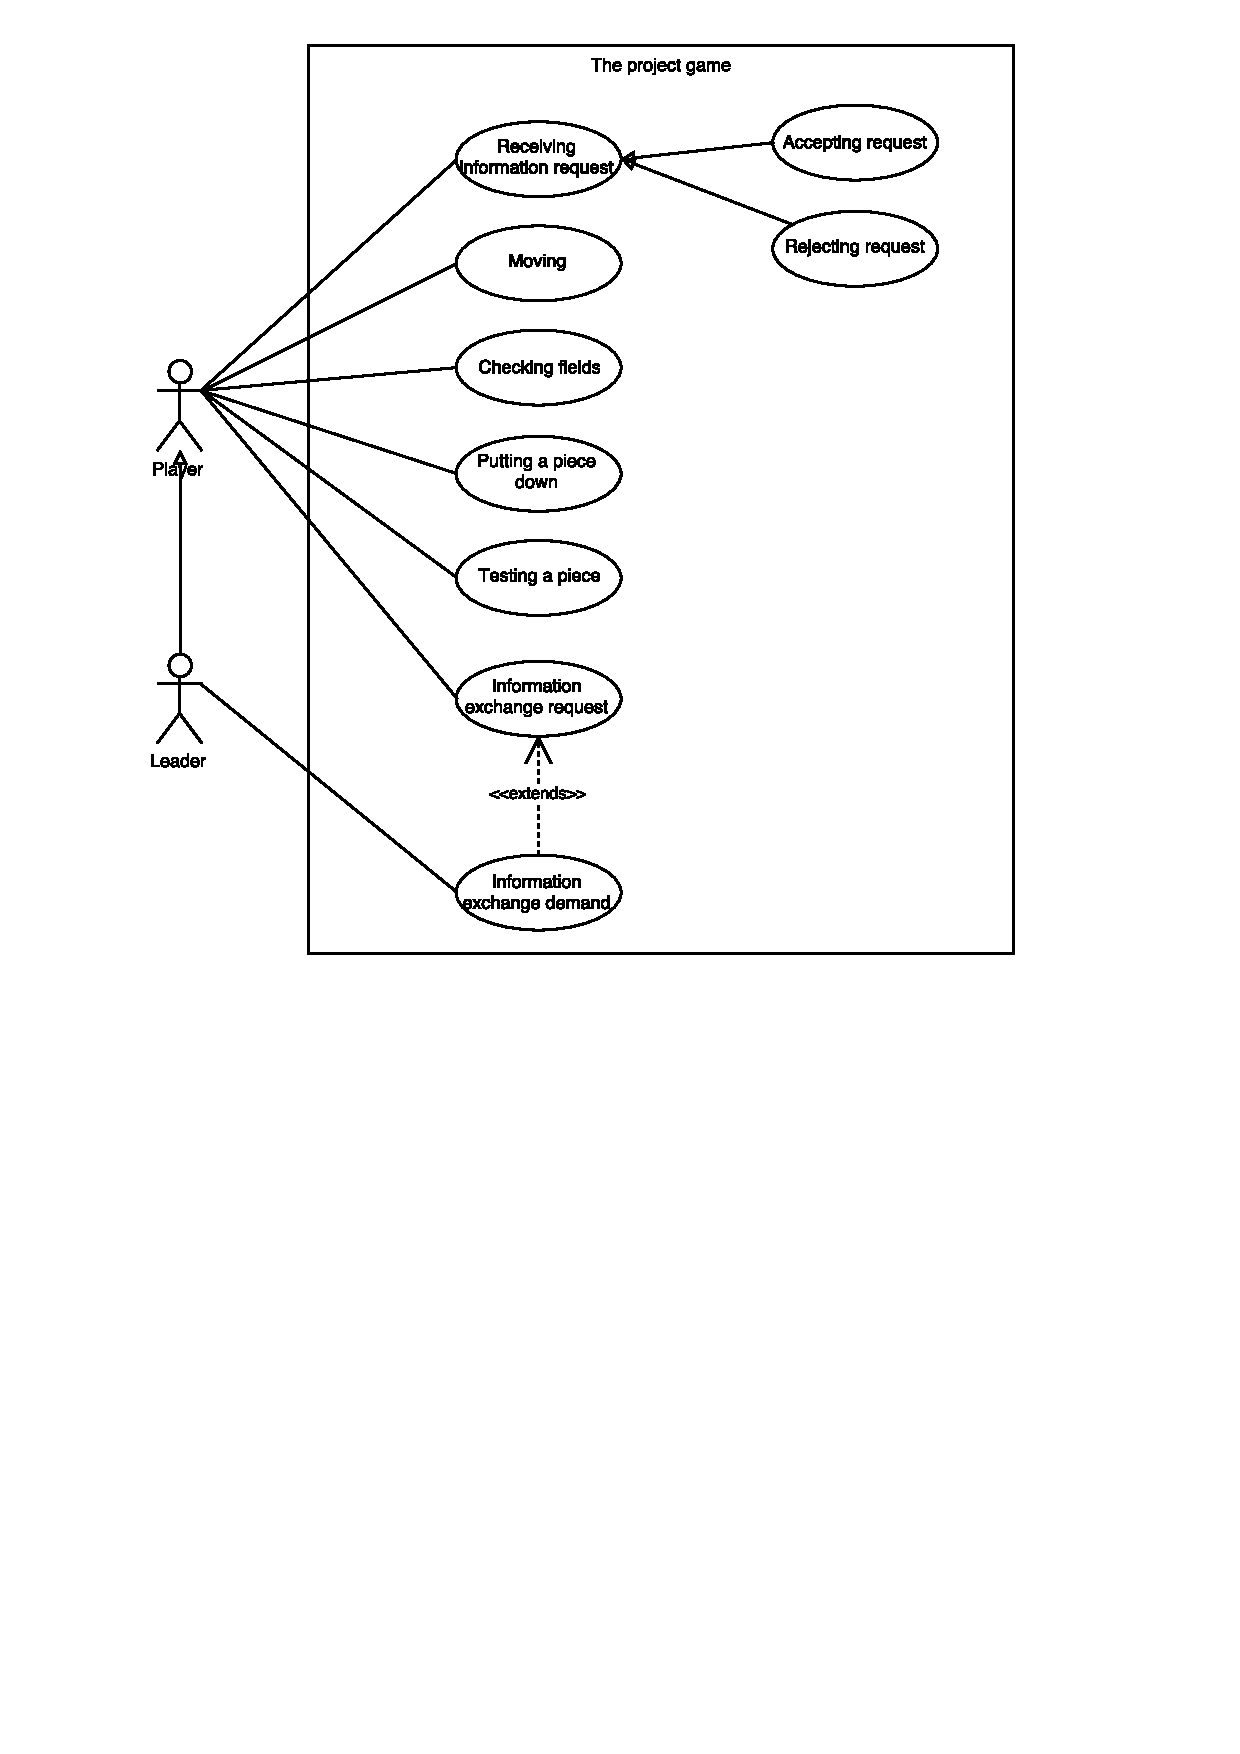
\includepdf[pages={1}]{przypadki_uzycia_gracz_lider.pdf}
A player may receive an information request. Then, they can accept or reject this request. A request from team leader cannot be rejected. The player can move in four directions, however they cannot enter goal area of the opposite team. They can check fields, pick up pieces located on them and test on goal area, whether the piece is real or a sham.  Player can request information exchange or demand it as a leader.
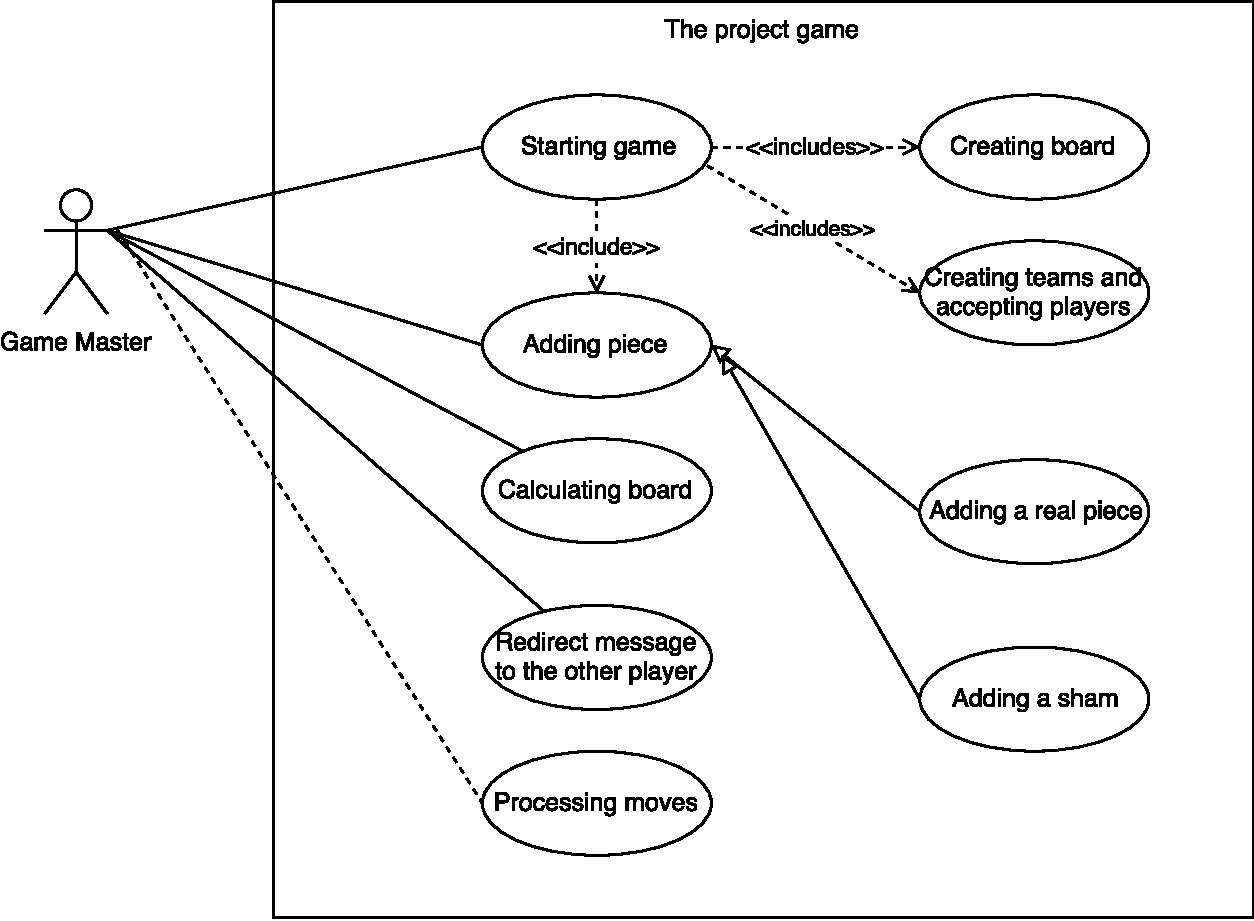
\includepdf[pages={1}]{przypadki_uzycia_gm.pdf}
Game Master starts a game, which include generating the Board, creating teams and accepting players. Then, during the game, it adds pieces to Task Area, which can be real pieces or shams, and calculate the Board. They also redirect messages between player and process their moves.
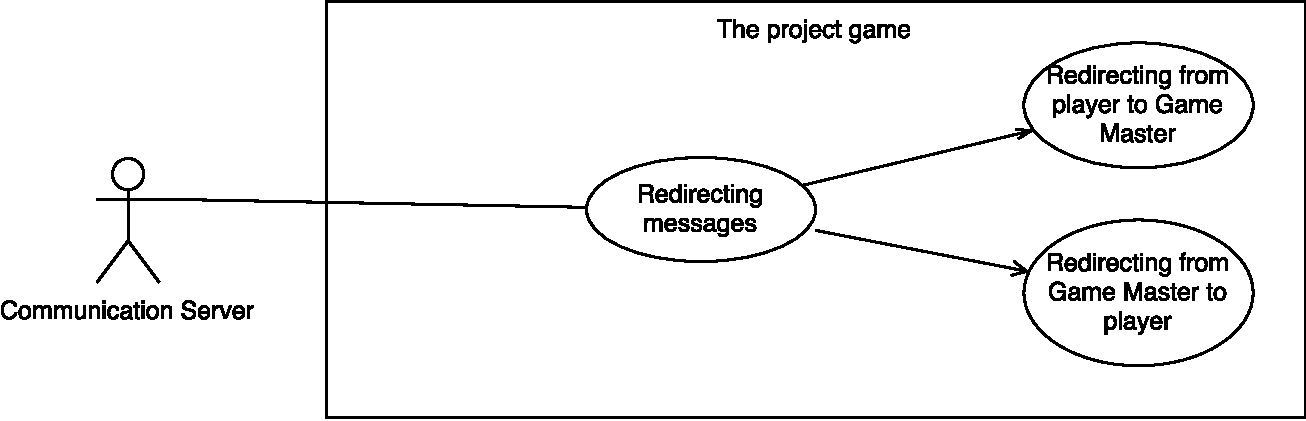
\includepdf[pages={1}]{przypadki_uzycia_cs.pdf}
Communication Server is responsible for redirecting messages between players and Game Master.
\newline
\section{Class diagram}
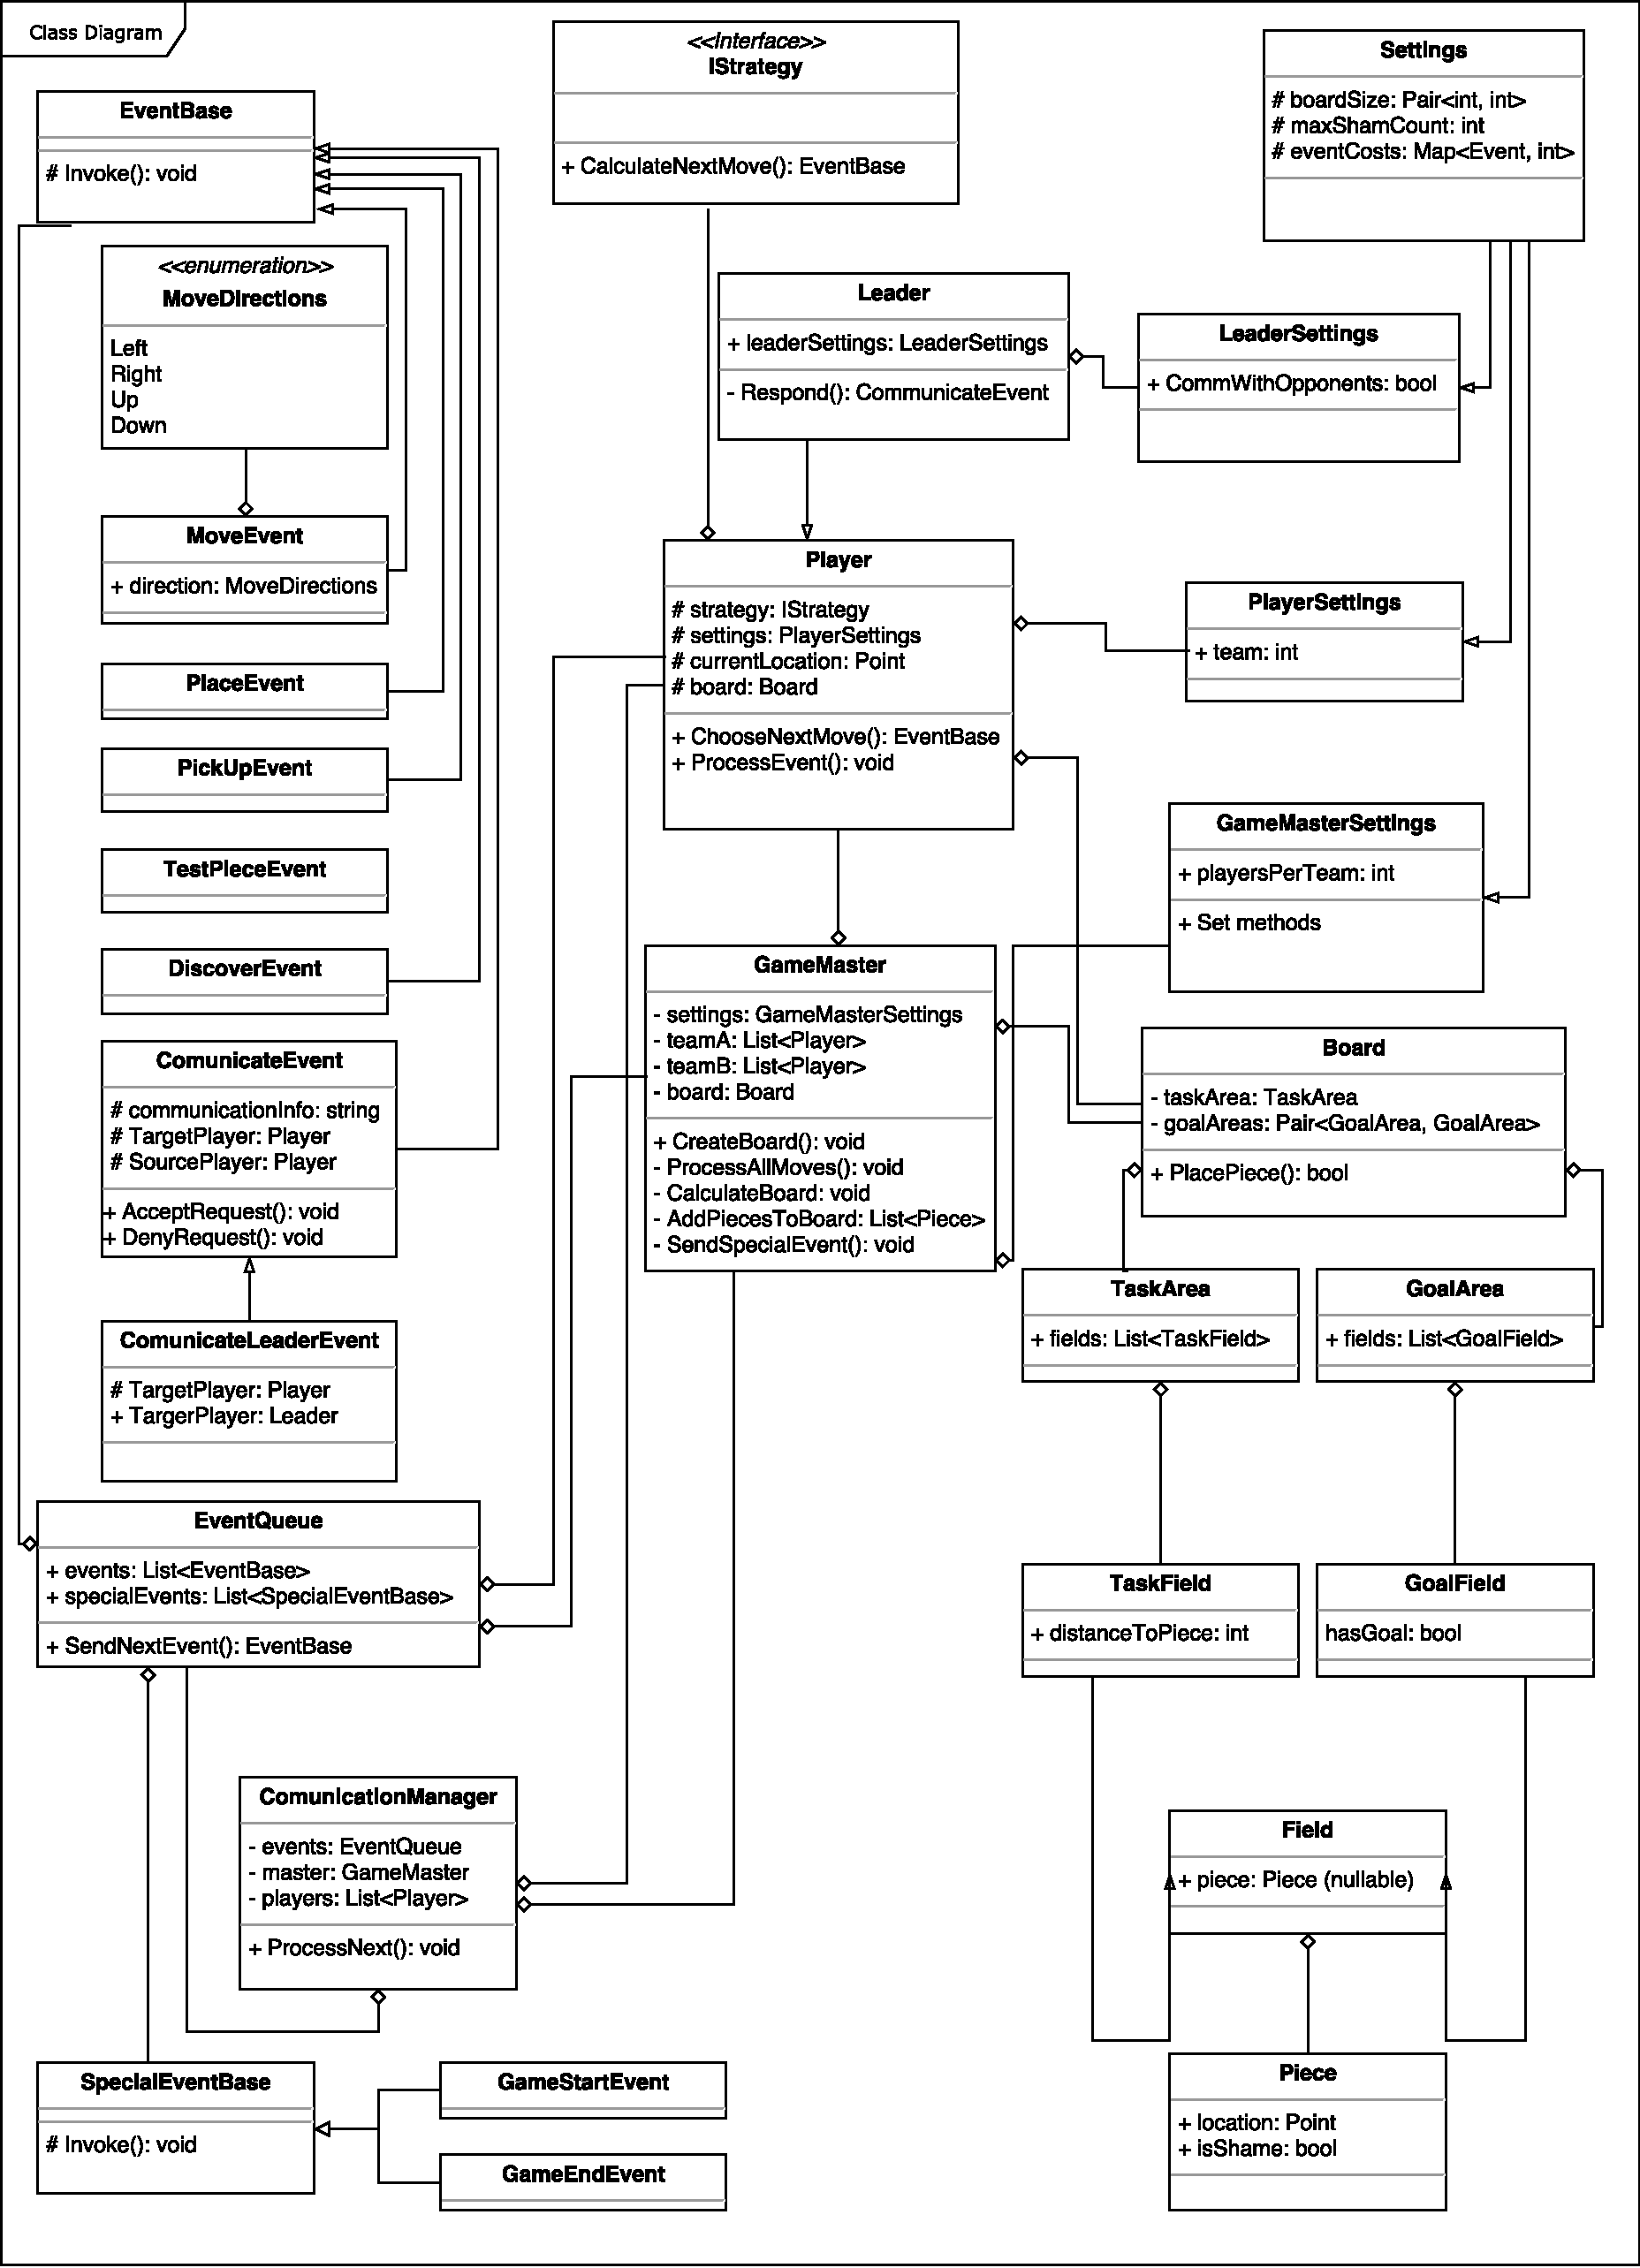
\includepdf[pages={1}]{diagram_klas.pdf}
Player class contains an strategy field , deciding about the strategy of a player – how their next move is calculated, settings field with an id of the team the player belongs to, field with their current location and a reference to the game board. Player can choose their next move and process events. Leader is a special type of player, having additional settings – whether they’ll communicate with opponents or not.
There are several events: MoveEvent, which includes an information about the move direction – Left, Right, Up or Down. There is a PickUpEvent and PlaceEvent, which happen when a piece is picked up or placed by a player; TestPieceEvent and DiscoverEvent – when player tests whether a piece is a sham or not and tries to discover a new goal; CommunicateEvent – contains information about player the message comes from, player being the target of the message and the message, as a string. Communication request can be rejected or accepted. Events are placed in EventQueue, which contains a list of regular events and special events – GameStartEvent and GameEndEvent.
GameMaster is the class responsible for creating the game board, calculating, adding pieces to it, processing all moves of players and sending special events about game start and end. This class has references to both teams and the board, it also has its settings object with an information about an amount of players in teams and set methods.
The communication between players and Game Master is passed through Communication Manager, which has a list of events, players and reference to Game Master.
The main settings class has an information about board size – a pair of integers defining its width and height, maximum number of pieces which may be shams and map of costs of every event.
The Board class contains three areas: one TaskArea, having a list of TaskFields and two GoalAreas with lists of GoalFields inside. Each Field contains a field with a piece, which can be set to null if there’s no piece on field. Additionally, TaskField has an information about the distance to the nearest piece and GoalField – information whether there’s a goal on it.
The Piece class has its location – a point on board and an information if it’s a sham or not.
\newpage
\section{Activity diagram}
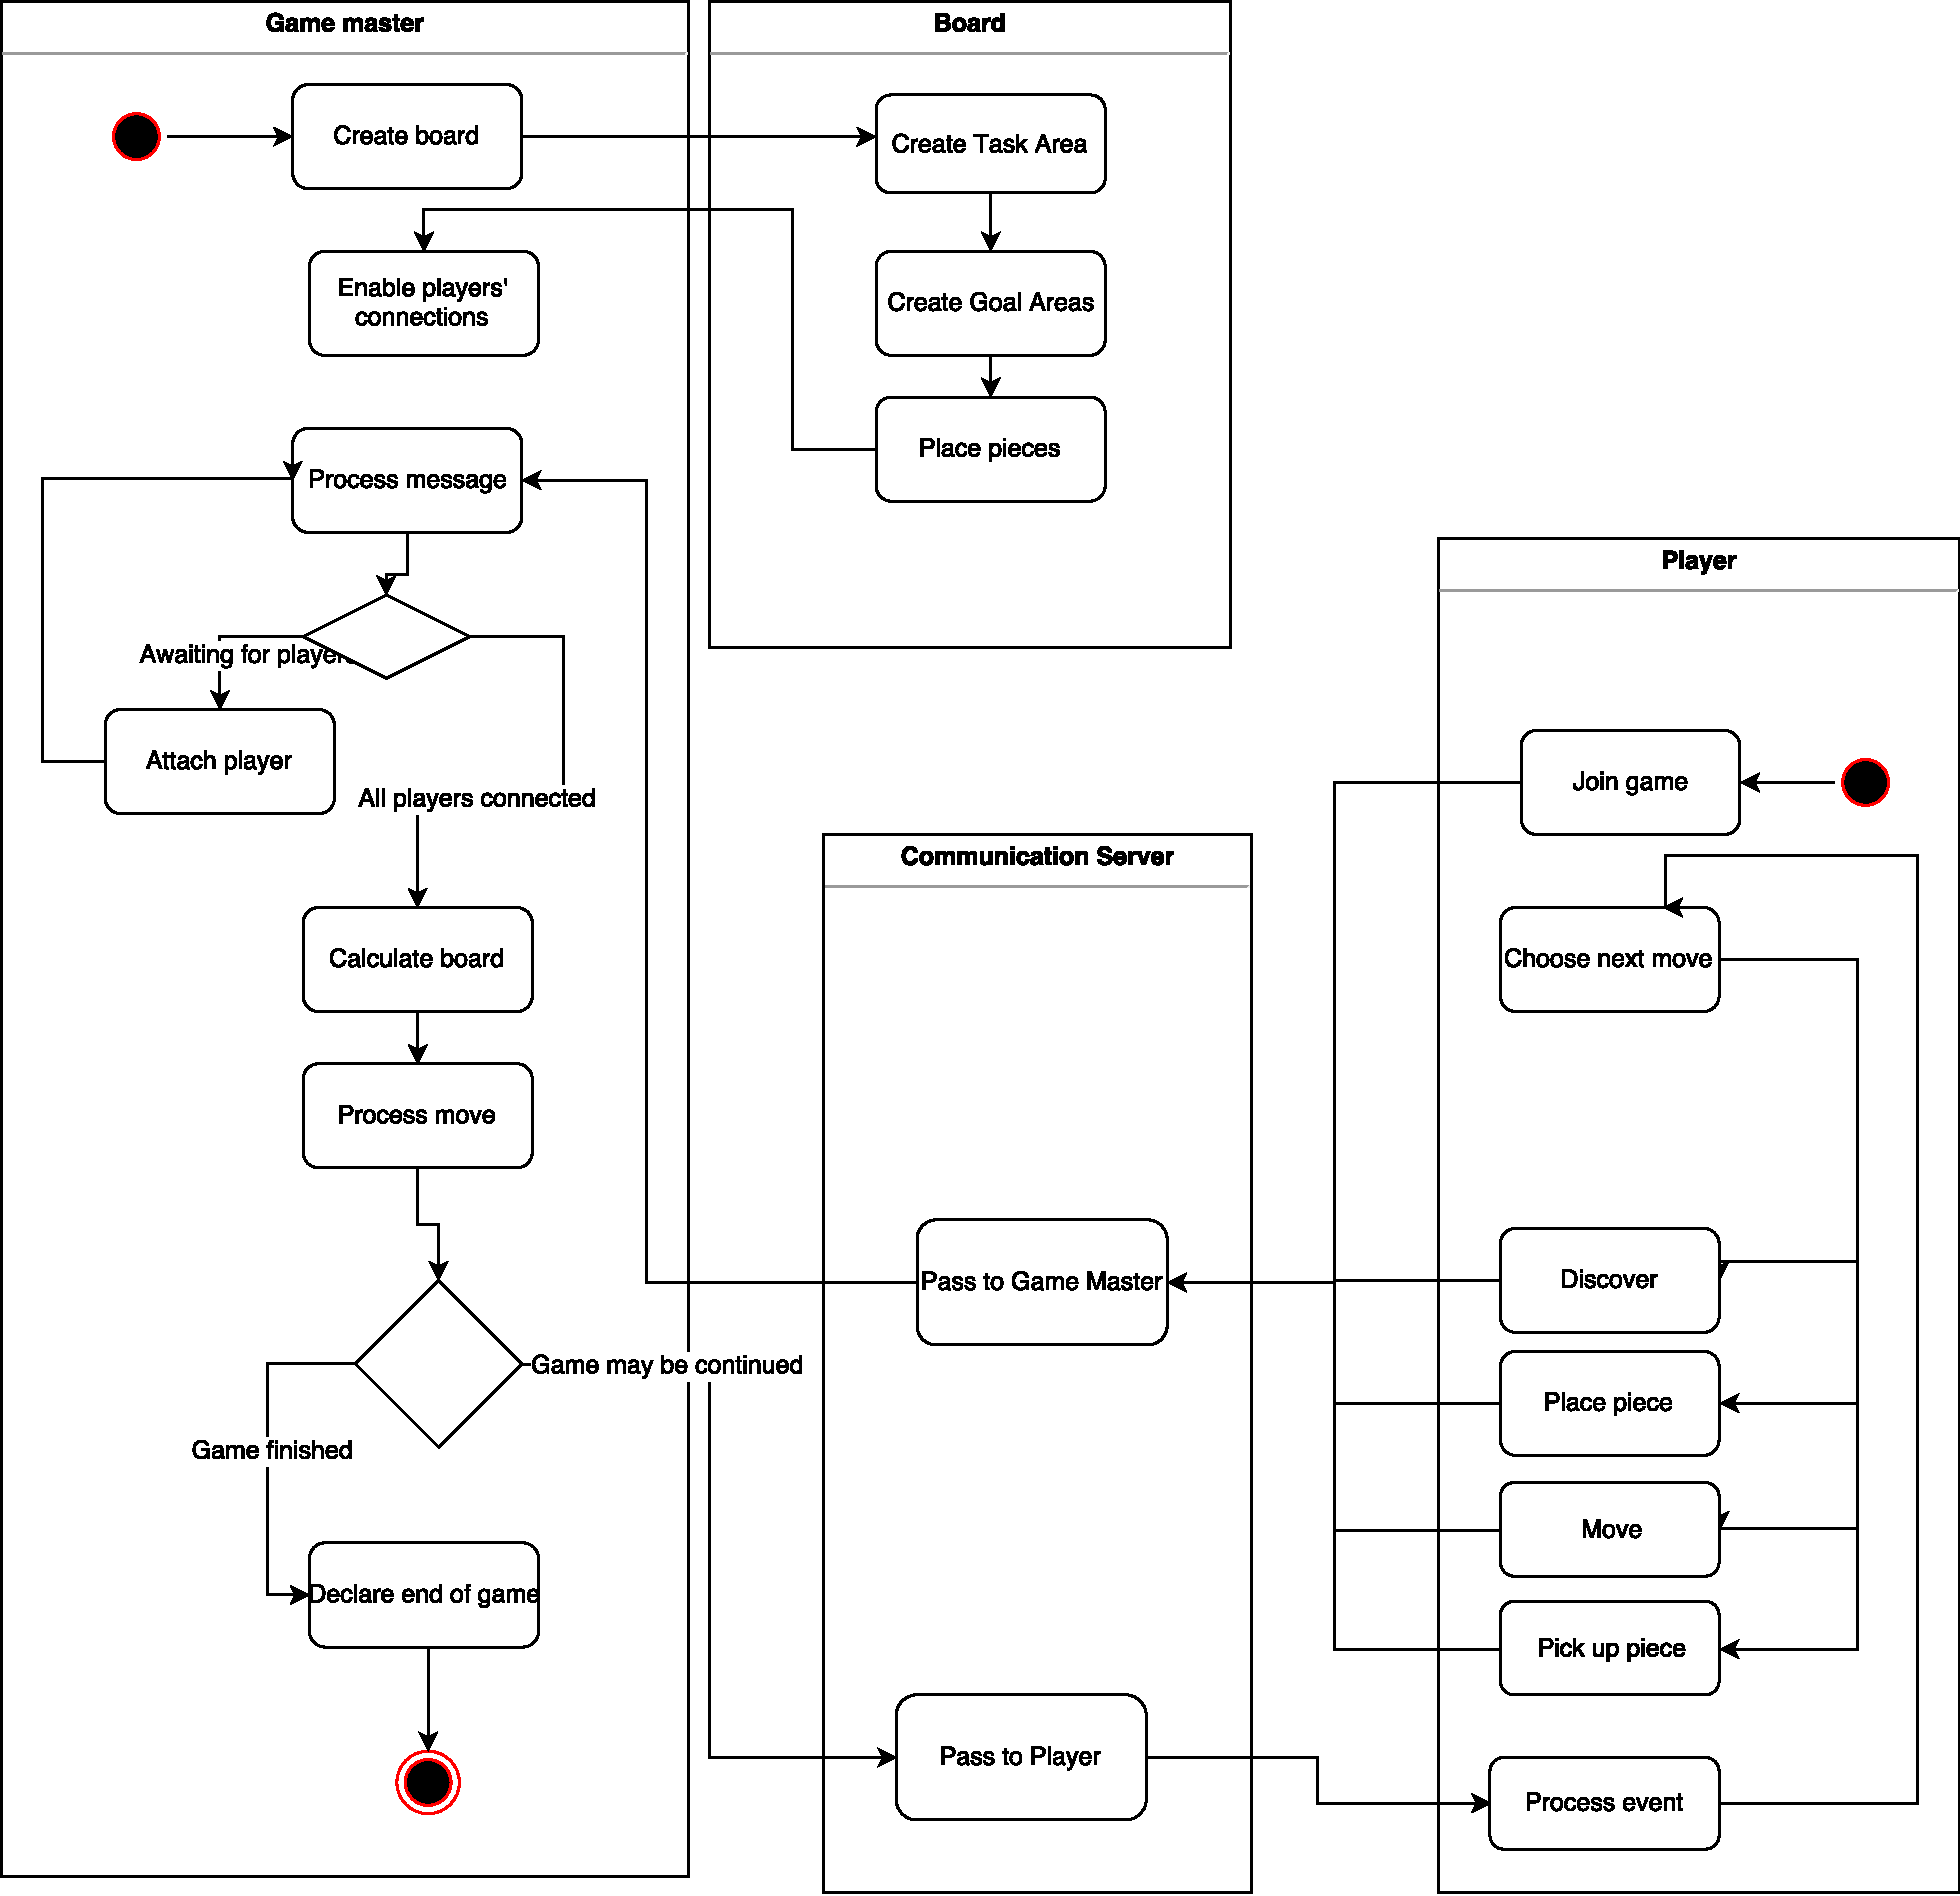
\includepdf[pages={1}]{diagram_aktywnosci.pdf}
Game is started. Game Master creates the Board: Task Area, Goal Areas and places pieces. Then it enables players' connections, waits for all player to connect and attaches them to teams. When all players are connected, Game Master calculate the Board and process players' moves. When the game is finished, it declares end of game.
Player may join a game and perform moves: discovering, placing piece, moving to other field and picking up piece. The move requests are passed to Game Master and sent back to player through Communication Server.
\newpage
\section{State diagram}
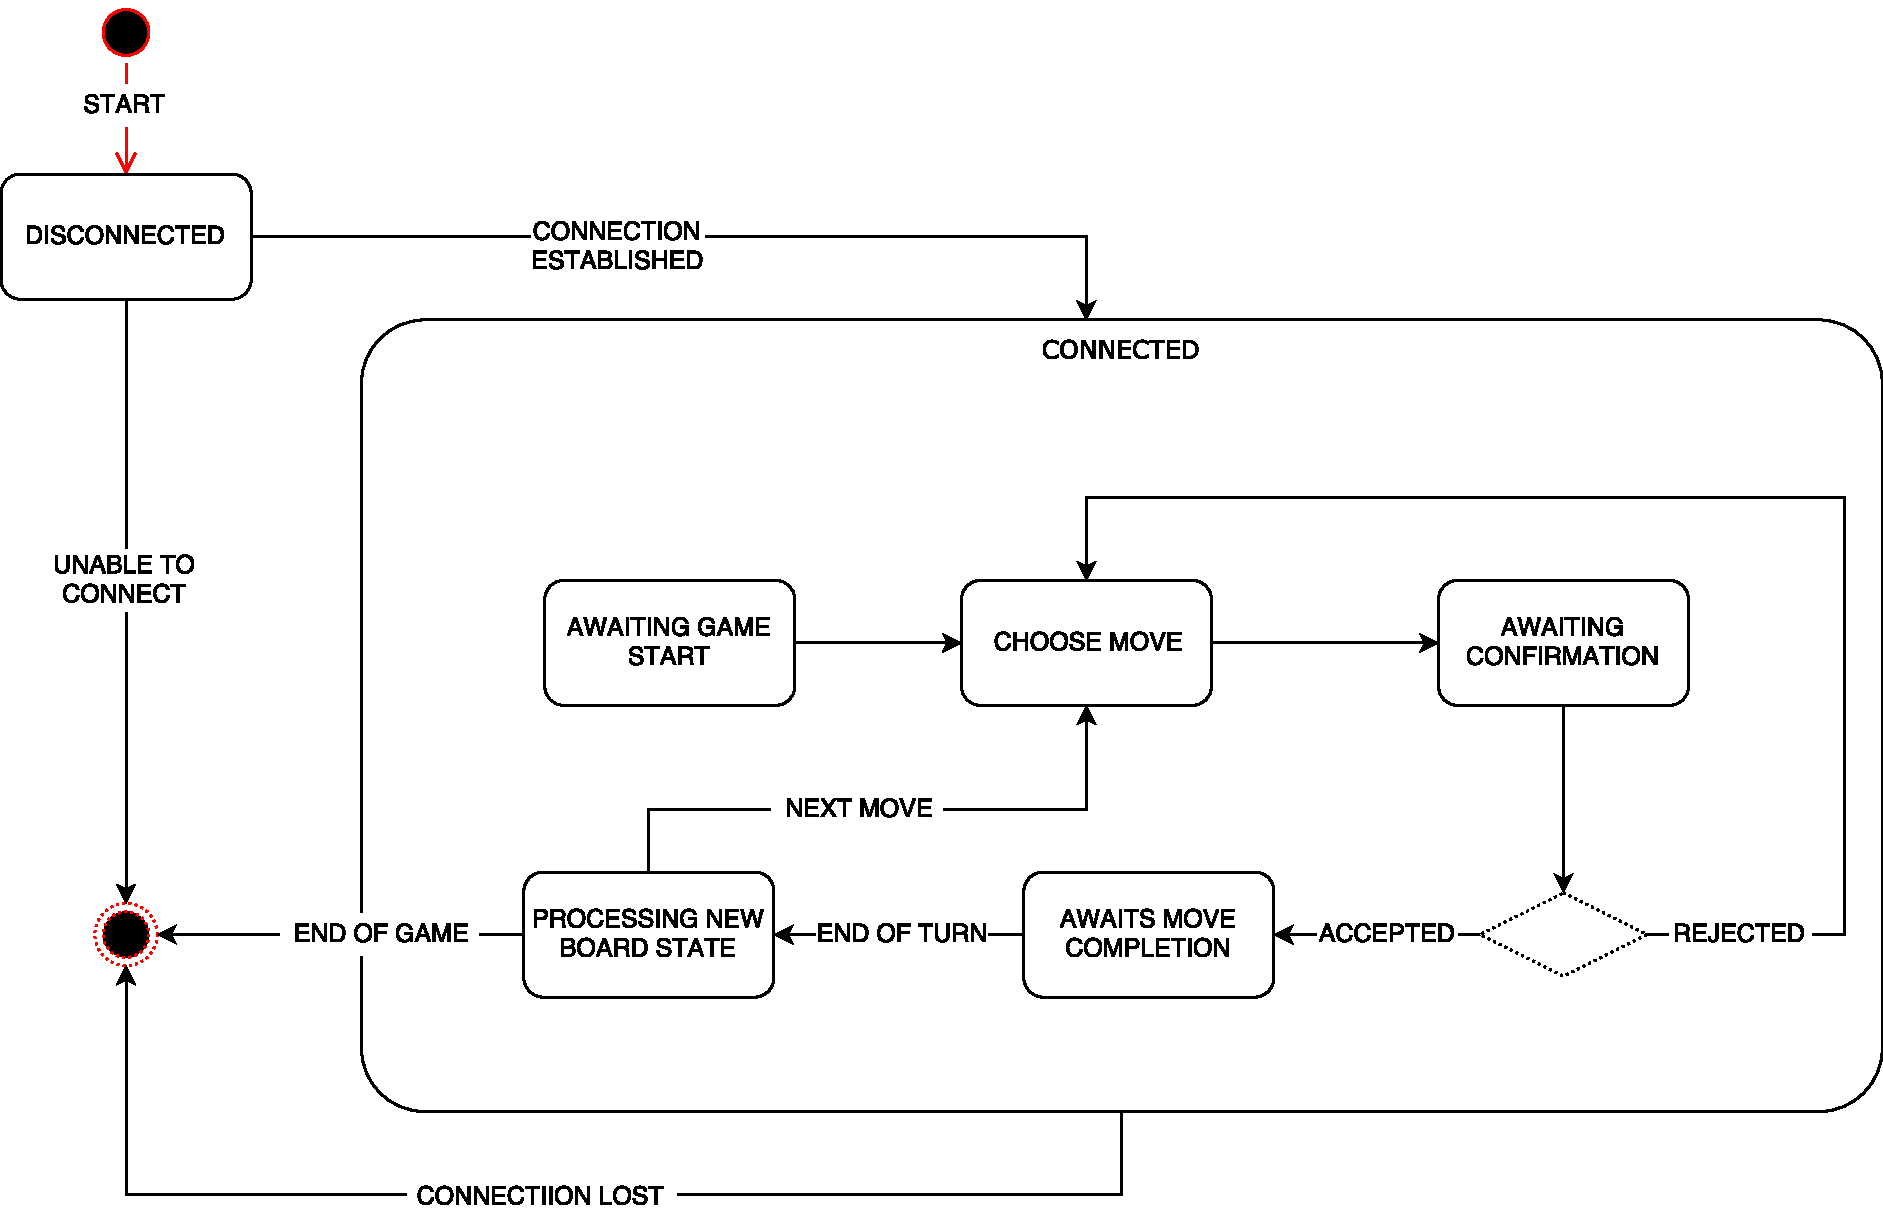
\includepdf[pages={1}]{state_diagram_player.pdf}
Player starts the game in DISCONNECTED state. Then it tries to establish a connection. If it's unable to do it, it terminates. When the connection is established, it awaits game start. When the game is started, the player needs to choose its next move. Then, it waits for confirmation from Game Master. If the move is rejected, it goes back to CHOOSE MOVE state. If it's accepted, player awaits move completion and after the end of turn, process new board state. It may now finish the Game, if Game Master tells it to do so, or choose its next move. If player loses connection, it terminates.
\newpage
\section{Sequence diagrams}
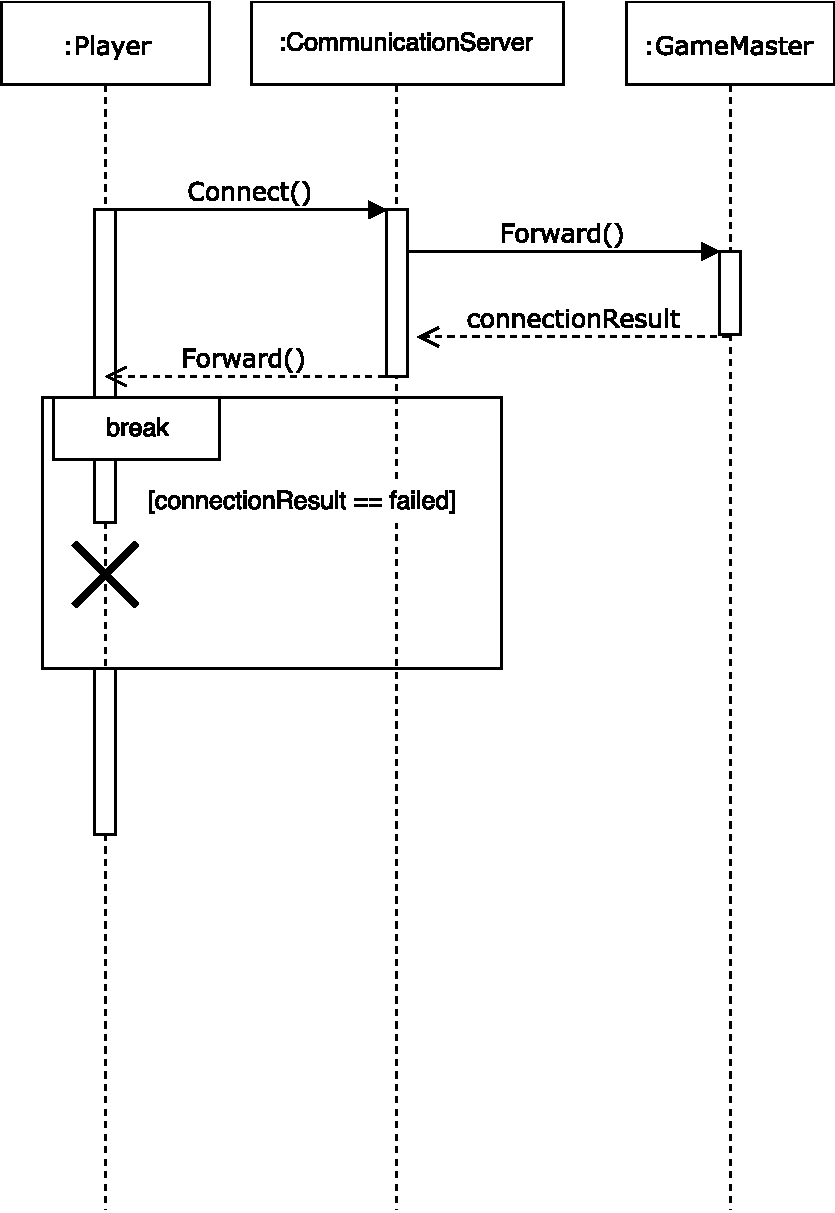
\includepdf[pages={1}]{sekwencje1.pdf}
Player firstly calls its Connect() method and waits for response from Communication Manager. It forwards the request to Game Master and waits for connection result to forward it to player. If player receive positive response, they participate in game. If connection result is negative, the player terminates.
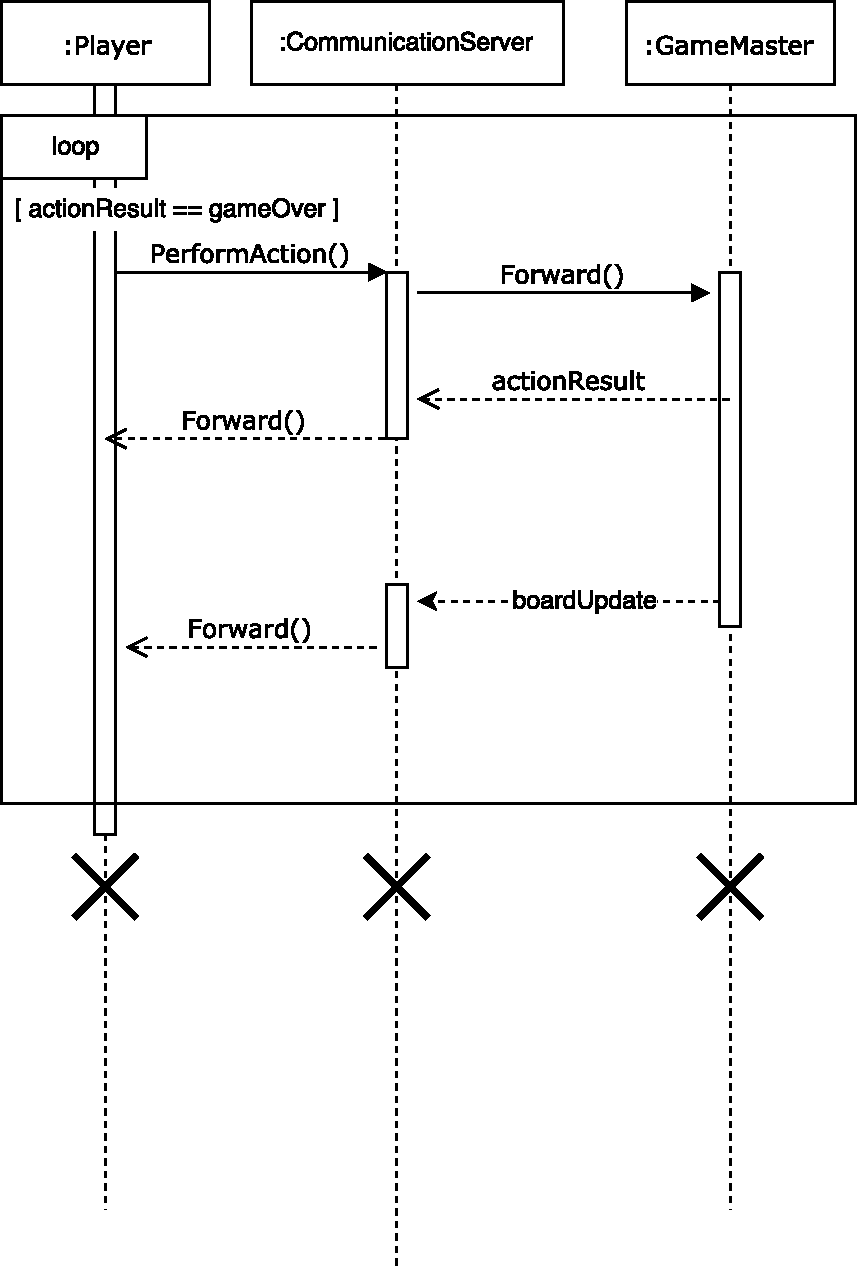
\includepdf[pages={1}]{sekwencje2.pdf}
Player performs actions in loop, which ends when action result forwarded to player by Communication Server equals "game over". The Communication Server is informed about actions performed by player and forwards them to Game Master, waits for action result and forward it to player. It also receives information about board updates from Game Master, which are forwarded to players.
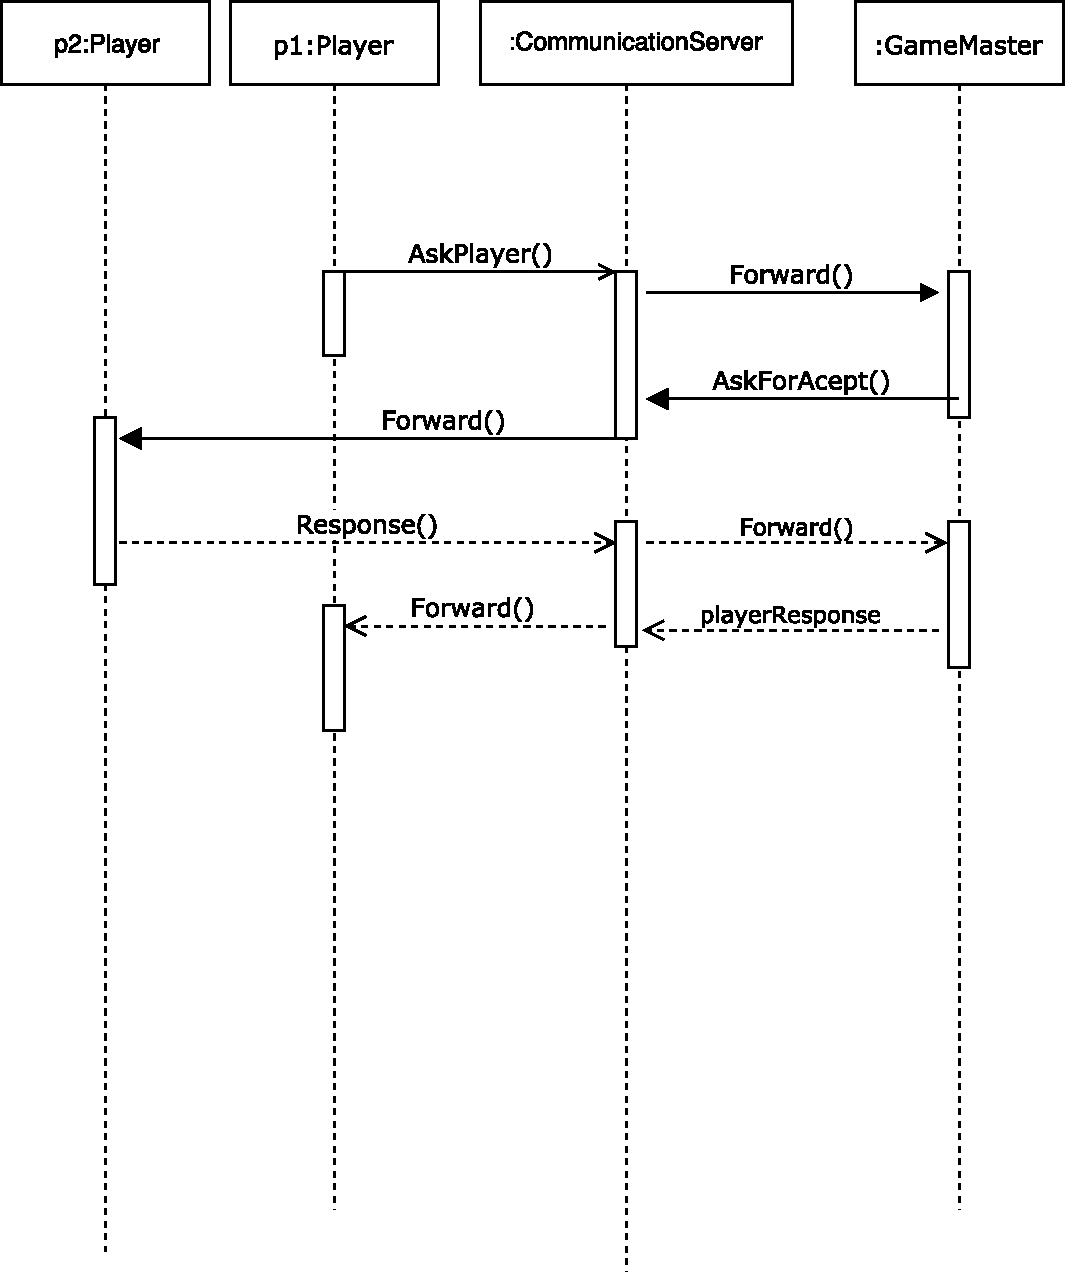
\includepdf[pages={1}]{sekwencje3.pdf}
The communication between players goes through Communication Server and Game Master. When Player p1 wants to ask Player p2, it firstly sends a message to Communication Server, which then asks the Game Master, whether the request from p1 to p2 shall be accepted. If so, the message from p1 is forwarded to p2. Player p2 may now send a response to message. It goes through Communication Server to Game Master, and the Game Master sends the response to Player p1 through Communication Server.


\end{document}
